
%% EE561_Report.tex
%% V1.0
%% 15-Dec-2014
%% by CyPhyNetS, LUMS
%% Support sites:
%% http://cyphnets.lums.edu.pk/
%% http://www.ctan.org/tex-archive/macros/latex/contrib/IEEEtran/
%% and
%% http://www.ieee.org/

\documentclass[conference]{IEEEtran}

\usepackage{latexsym}
\usepackage{amsmath}
\usepackage{amssymb}
\usepackage{amsthm}
\usepackage{epsfig}
\usepackage{courier}
\usepackage[usenames,dvipsnames]{color}
%\usepackage{ulem}
\usepackage{graphicx}
\usepackage{layout}
\usepackage{enumerate}
%\usepackage{manfnt}
%\usepackage{arabtex}
\usepackage{mathrsfs}
\usepackage[setpagesize=false]{hyperref}

\parskip 0.5ex
\begin{document}
%
% paper title
% can use linebreaks \\ within to get better formatting as desired
\title{Trajectory Analysis and Optimum Control of Differential Drive Robot}
\author{\IEEEauthorblockN{Hassan, Danial}
\IEEEauthorblockA{Department of Electrical Engineering\\
SBA School of Science \& Engineering, LUMS\\
Lahore, Pakistan\\
\{15100063, 15100177\}@lums.edu.pk}}
\maketitle
\begin{abstract}
%\boldmath
A novel control design of a differential robot has been presented in this paper. Discussion starts with the introduction of the kinematic model of a differential 
robot. Using this kinematic model a state space is designed, for the differential robot, which uses the error of the robot from the reference as the state of the system
Then, a controller is designed which is used to control the robot to follow the reference path with minimal error. Finally, simulations are carried out to see how
tightly the robot follows the given trajectory, with and without error, as compared to the open loop case. The results of the simulations show the applicability of the
given algorithm for the differential drives
\end{abstract}

\begin{keywords}
digital control systems; differential drive; trajectory tracking; bestProjectEver; 
\end{keywords}

\IEEEpeerreviewmaketitle
\section{Introduction}
% no \IEEEPARstart
Differential robot is one of the most used robot in robotics because of its ease of use \cite{papadopoulos2007differential}. This paper deals with the trajectory analysis of a differential robot in open loop
and then in closed loop along with the design of a linear controller to control it in closed loop. The robot is provided with a reference trajectory. It uses that  trajectory
to find reference tangential and angular speed at each point and the error is calculated between the reference and the actual trajectory to see how tightly the robot follows
the given path. Also it is assumed the the path of the robot is obstacle free to see the accuracy of the robot and the designed controller in following the reference path.
Along with this, the robot is also made to follow the reference path in closed loop under noisy conditions for comparison purposes. The paper follows the following flow. First,
the differential model of the robot is found. Then, state space design of the given robot is derived followed by derivation of control law, controllability and reference input.Finally,
the algorithm is presented to control the robot followed by simulations and conclusion.
%%%%%%%%%%%%%%%%%%%%%%%%%%%%%%%%%%%%%%%%%%%%%%%%%%%%%%%%%%%%%
\section{Methodology}
We start by deriving forward and reverse kinematics equations for a differential drive robot \cite{de1995modelling}. These equations are used to design an open loop controller for the robots to follow a reference trajectory. This open loop controller takes in series of values of $x_{r}$ and $y_{r}$ coordinates on the reference path and outputs (feed-forward) linear and angular velocities ($v_{ff}$ and $\omega_{ff}$ respectively) to be feed to the robot. Response of the robot using the open loop controller is studied and its limitations are identified.

Next a feedback loop is added to the already developed feedforward controller for robust trajectory tracking and noise rejection. An equation for the error in tracking is derived in the frame of the robot using a coordinate transformations. Finally a state state equation of error is obtained by linearizing the system.

Conditions of controllability of the error are found using the rank of controllability matrix. Finally a control law is designed using appropriate gains, overshoot, settling time etc. The designed controller is rigorously tested and the simulation results are attached in the document.
\subsection{Mathematical Model}
We start with the kinematic model of the differential in which we provide its direct and inverse kinematics. Fig??????? shows the model of the robot along with symbols.
The motion of equations of motion of the robot are as follows.
\begin{equation}\label{eq}
\begin{bmatrix}
\dot{x_{c}}\\ 
\dot{y_{c}}\\ 
\dot{\theta_{c}}
\end{bmatrix}
=
\begin{bmatrix}
cos(\theta) & 0\\ 
sin(\theta) & 0\\
0 & 1
\end{bmatrix}
\cdot 
\begin{bmatrix}
v\\
w
\end{bmatrix}
\end{equation}
where v and w are the tangential and angular velocities of the robot respectively.
Since we do not have direct access of the v and w of a differential drive robot, we must vary the speeds of right and left motors to maintain the required linear and angular velocities. 
Circumferential velocities of the right and left wheels of the robot can be derived from the $v$ and $\omega$ using the following equations:
\begin{equation}\label{eq}
v_{r} = v + \frac{wL}{2}
\end{equation}
\begin{equation}\label{eq}
v_{l} = v - \frac{wL}{2}
\end{equation}
L here is the wheel track of the robot.

\subsection{Feedforward Control}
For given sets of points that define the reference trajectory $ (x_{r} , y_{r}) $, a feed forward control law can be derived \cite{chung2001position}. Inverse kinematics equations derived for the differential drive robot can be used to calculate the robot inputs, the tangential velocity and angular velocity. By varying these parameters in accordance to the reference path, the robot can be made to follow the required path perfectly given there are no disturbances and robot starts with zero initial state error.

The tangential velocity of the reference path denoted by $v_{r}$ is given by:
\begin{equation}\label{eq}
v_{r} = \sqrt{\dot{x_{r}^{2}} + \dot{y_{r}^{2}}}
\end{equation}
The tangent angle $\theta_{r}$ of each point on the path is obtained from:
\begin{equation}\label{eq}
\theta_{r} = tan^{-1}(\frac{\dot{y_{r}}}{\dot{{x_{r}}}}) + k\pi
\end{equation}
By calculating the time derivative of above equation angular velocity $w_{r}$ of the path can be determined.
\begin{equation}\label{eq}
w_{r} = \frac{\mathrm{d} \theta_{r}}{\mathrm{d} t} = \frac{\dot{x_{r}}\ddot{y_{r}} - \dot{y_{r}}\ddot{x_{r}}}{\dot{x_{r}}^{2}+\dot{y_{r}}^{2}}
\end{equation}
If the robot is placed at the start of the path with correct orientation and the linear and angular velocities of the robot are made equal to that of the reference path
\begin{equation}\label{eq}
v_{robot} = v_{r}  \;\;\;\;  w_{robot} = w_{r}
\end{equation}
the robot can be made to trace the reference path exactly in the absence of noise.

Through out the rest of this document these tangential and angular velocities will be refereed to as robot's feed-forward tangential $v_{ff}$ and feed-forward angular velocities $\omega_{ff}$ respectively,
%%%%%%%%%%%%%%%%%%%%%%%%%%%%%%%%%%
\subsection{Block Diagram}
The block diagram in fig 1 shows the feedback and feedforward loops. The output of feedforward block is called $v_{ff}$ and $\omega_{ff}$.
The output of feedback block is called $v_{b}$ and $\omega_{b}$. And the input to the robot that is the sum of feedback and feedforward velocities is called $v$ and $\omega$.
\begin{figure}[!t]
\centering
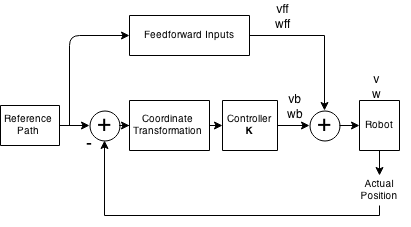
\includegraphics[scale=0.63]{block_diagram}
\caption{Feedback block diagram.}
\end{figure}
%%%%%%%%%%%%%%%%%%%%%%%%%%%%%%%%%%
\subsection{Feedback Control}
When the robot is controlled to follow a give reference trajectory, there will always be error in tangential and angular velocity given no ideal conditions.The 
method in the design of the controller starts by determining error in the actual and reference trajectory of the robot. This error is then used as the state space 
model of the differential robot. The aim is to control the robot such that the error approaches zero.The error
is calculated in the reference of the robot and is as follows: 


\begin{figure}[!t]
\centering
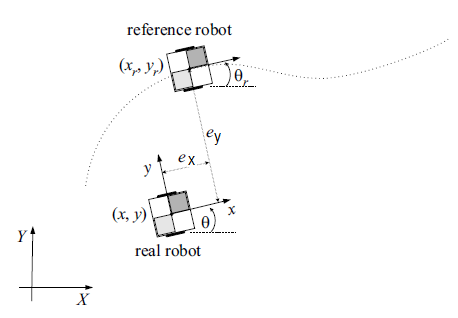
\includegraphics[scale=0.6]{transformation}
\caption{Error calculation in real robot frame \cite{XingPGuo}}
\end{figure}

\begin{equation}\label{eq}
\begin{bmatrix}
e_{x}\\ 
e_{y}\\ 
e_{\theta}
\end{bmatrix}
=
\begin{bmatrix}
cos(\theta) & sin(\theta) & 0\\ 
-sin(\theta) & cos(\theta) & 0\\ 
0 & 0 & 1
\end{bmatrix}
\cdot
\begin{bmatrix}
x_{r}-x\\ 
y_{r}-y\\ 
\theta_{r}-\theta
\end{bmatrix}
\end{equation}

Derivating the above equation to obtain $\dot{e}$
\begin{equation}\label{eeq}
\begin{split}
\begin{bmatrix}
\dot{e_{x}}\\ 
\dot{e_{y}}\\ 
\dot{e_{\theta}}
\end{bmatrix}
=
\begin{bmatrix}
-sin(\theta) & cos(\theta) & 0\\ 
-cos(\theta) & -sin(\theta) & 0\\ 
0 & 0 & 1
\end{bmatrix}
\cdot
\begin{bmatrix}
x_{r}-x\\ 
y_{r}-y\\ 
\theta_{r}-\theta
\end{bmatrix}
+\\
\begin{bmatrix}
cos(\theta) & sin(\theta) & 0\\ 
-sin(\theta) & cos(\theta) & 0\\ 
0 & 0 & 1
\end{bmatrix}
\cdot
\begin{bmatrix}
V_{r}-x\\ 
V_{r}-y\\ 
\theta_{r}-\theta
\end{bmatrix}
\end{split}
\end{equation}

Using the robot kinematics equation (1) above equation can be written as
\begin{equation}\label{eeq}
\begin{split}
\begin{bmatrix}
\dot{e_{x}}\\ 
\dot{e_{y}}\\ 
\dot{e_{\theta}}
\end{bmatrix}
=
\begin{bmatrix}
cos(e_{\theta}) & 0\\ 
-sin(e_{\theta}) & 0\\ 
0 & 1
\end{bmatrix}
\cdot
\begin{bmatrix}
v_{ff}\\ 
\omega_{ff}
\end{bmatrix}
+\\
\begin{bmatrix}
-1 & e_{y}\\ 
0 & -e_{x}\\ 
0 & -1
\end{bmatrix}
\cdot
\begin{bmatrix}
v\\ 
\omega
\end{bmatrix}
\end{split}
\end{equation}

Where the terms $v$ and $\omega$ that arrived from the differentiation of the $x$ and $y$ terms in (9), are the inputs to the our robot. From the feedback and feedforward loops that we proposed in the blockdiagram fig 1, $v$ and $\omega$ can be written as 
\begin{equation}\label{eq}
v = v_{ff} + v_{b}
\end{equation}
\begin{equation}\label{eq}
\omega = \omega_{ff} + \omega_{b}
\end{equation}

Substituting the values of $v$ and $\omega$ from (11) and (12) into (10) to obtain the error equation in terms of the closed loop inputs takes us one step further to the standard state space form of equation
\begin{equation}\label{eq}
\begin{split}
\begin{bmatrix}
\dot{e_{x}}\\ 
\dot{e_{y}}\\ 
\dot{e_{\theta}}
\end{bmatrix}
=
\begin{bmatrix}
0 & \omega_{ff} & 0\\ 
-\omega_{ff} & 0 & 0\\ 
0 & 0 & 0
\end{bmatrix}
\cdot 
\begin{bmatrix}
e_{x}\\ 
e_{y}\\ 
e_{\theta}
\end{bmatrix}
+
\begin{bmatrix}
-1 & 0\\ 
0 & 0\\
0 & -1
\end{bmatrix}
\cdot 
v_{b} \\
+
\begin{bmatrix}
cos(e_{\theta}) & 0\\ 
sin(e_{\theta}) & 0\\
0 & 1
\end{bmatrix}
\cdot 
\begin{bmatrix}
v_{ff}\\
\omega_{ff}
\end{bmatrix}
\end{split}
\end{equation}

\subsection{Linearization and State Space Model}
If the controller is effective, then the robot will follow the given reference trajectory very effectively and there will be minimal error. Hence, linearizing the equation around our operating point
\[
e_{x}=e_{y}=e_{\theta}=0 \;,\;
\]
we get results in state space equation of the form $\dot{e}=F.e+G.U$.
\begin{equation}\label{eq}
\begin{bmatrix}
\dot{e_{x}}\\ 
\dot{e_{y}}\\ 
\dot{e_{\theta}}
\end{bmatrix}
=
\begin{bmatrix}
0 & \omega_{ff} & 0\\ 
-\omega_{ff} & 0 & v_{ff}\\ 
0 & 0 & 0
\end{bmatrix}
\cdot 
\begin{bmatrix}
e_{x}\\ 
e_{y}\\ 
e_{\theta}
\end{bmatrix}
+
\begin{bmatrix}
-1 & 0\\ 
0 & 0\\
0 & -1
\end{bmatrix}
\cdot 
v_{b}
\end{equation}

\subsection{Controller Design}
\subsubsection{Controllability}
Now that the equation of the error is in state space form ($ \mathbf{\dot{e} = F \cdot e + G \cdot u} $) we can determine the controllability of our state using the rank of $C$ matrix.
\begin{equation}\label{eq}
C = 
\begin{bmatrix}
1 & 0 & 0       & 0& -\omega_{ff}^{2} & \omega_{ff}\cdot v_{ff}\\ 
0 & 0 & -\omega_{ff} & v_{ff}        & 0          & 0\\ 
0 & 1 & 0       & 0& 0          & 0
\end{bmatrix}
\end{equation}
$\mathbf{ rank(C) = 3 }$ as long as $v_{ff}$ and $\omega_{ff}$ are not both zero.

\subsubsection{Gain Matrix}
Our system has 3 states ($ e_{x},e_{y},e_{\theta}$) and 2 inputs ($v_{b},\omega_{b}$) so according to the equation
\begin{equation}\label{eq}
V=K\cdot e
\end{equation}
the dimensions of the gain matrix $\mathbf{K}$ must be 2x3.

The general structure of the gain matrix can be intuitively found out using fig 1. Varying the angular velocity $\omega_{b}$ of the robot has no effect on the tangential error $e_{x}$, so this must be catered by controlling the tangential velocity $v_{b}$. Similarly the tangential velocity has no effect on the orthogonal error $e_{y}$ and orientation error $e_{\theta}$. These errors must be reduced by manipulating the angular velocity. Using the intuitions above the gain matrix comes out like this

\begin{equation}\label{eq}
\begin{bmatrix}
v_{b}\\ 
\omega_{b}
\end{bmatrix}
=
\begin{bmatrix}
k_{x} & 0 & 0\\ 
0 & k_{y} & k_{\theta}
\end{bmatrix}
\cdot 
\begin{bmatrix}
e_{x}\\ 
e_{y}\\ 
e_{\theta}
\end{bmatrix}
\end{equation}

The characteristic equation of a closed loop is given by
\begin{equation}\label{eq}
\begin{split}
det(s\boldsymbol{I-F+GK})=s^3+(k_{x}+k_{\theta})s^2+ \\
(k_{x}k_{\theta}+k_{y}v_{ff}+\omega_{ff}^2)s+k_{x}k_{y}v_{ff}+k_{\theta}\omega_{ff}^2
\end{split}
\end{equation}

We can design the controller by calculating the value of gains that makes the polynomial in eq (18) equal to desired characteristic polynomial. A third order polynomial takes the form of
\begin{equation}\label{eq}
(s+\alpha\zeta\omega_{n})(s^2+2\zeta\omega_{n}+\omega_{n}^2)
\end{equation}

By comparing the coefficients in Eqs (18) and (19), gains $k_{x}, k_{y}, k_{\theta}$ can be expressed in terms of $\zeta$ and $\omega_{n}$ and $\alpha$ as
\begin{equation}\label{eq}
\begin{split}
k_{x}+k_{\theta}= (\alpha+2)\zeta\omega_{n}\\
k_{x}k_{\theta}+k_{y}v_{ff}+\omega_{ff}^2= 2\alpha\zeta^2\omega_{n}^2+\omega_{n}^2\\
k_{x}k_{y}v_{ff}+k_{\theta}\omega_{ff}^2= \alpha\zeta\omega_{n}^3
\end{split}
\end{equation}

Equations (20) can be solved simultaneously on matlab using the $solve$ command. The equation was solved using many possible values of $\alpha$ and the most elegant solution obtained by putting $\alpha = 2$ is
\begin{equation}\label{eq}
\begin{split}
k_{x} = 2\zeta\omega_{n} \\
k_{\theta} = 2\zeta\omega_{n} \\
k_{y} = \frac{\omega_{n}^2-\omega_{ff}^2}{v_{ff}}
\end{split}
\end{equation}

The response of the error was designed for a Maximum Overshoot of 5\% and Settling Time of 2s that resulted from the following values of $\zeta$ and $\omega_{n}$
\begin{equation}\label{eq}
\begin{split}
\zeta = 0.6901 \\
\omega_{n} = 3.3328 \\
\end{split}
\end{equation}

But since the system is third order and the third pole is close to $jw$ axis, actual characteristics of the error are a little different. As obtained from matlab $stepinfo$ command the actual performance indicators of the system are below
\begin{equation}
\begin{split}
RiseTime: 0.7770 \\
SettlingTime: 1.9784 \\
SettlingMin: 0.0176 \\
SettlingMax: 0.0202 \\
Overshoot: 3.1375 \\
Undershoot: 0.0000 \\
Peak: 0.0202 \\
PeakTime: 1.6418
\end{split}
\end{equation}

and the values of the gains obtained of such a system are

\begin{equation}\label{eq}
\begin{split}
k_{x} = 4.6000 \\
k_{\theta} = 4.6000 \\
k_{y} = \frac{11.1077-\omega_{ff}^2}{v_{ff}}
\end{split}
\end{equation}

these gains were used for simulations.
\begin{figure}[h!]
  \caption{Close Loop with Noise, without Zero Error}
  \centering
    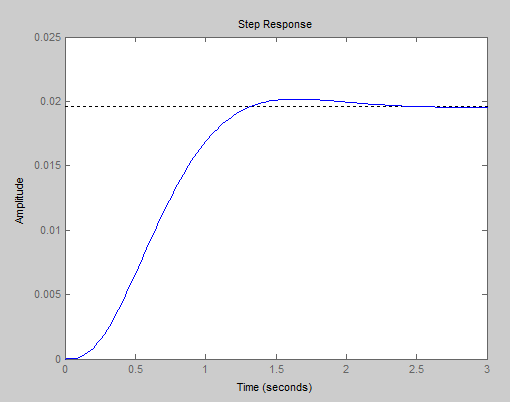
\includegraphics[width=0.5\textwidth]{response}
\end{figure}
%%%%%%%%%%%%%%%%%%%%%%%%%%%%%%%%%%
\section{Simulations \& Experiments}
Figures 3,4,5,6 shows the results of the simulation using feedforward (open loop) and feedback (closed loop) controller designed in this paper.
\begin{figure}[h!]
  \caption{Open Loop with Zero Error, without Noise}
  \centering
    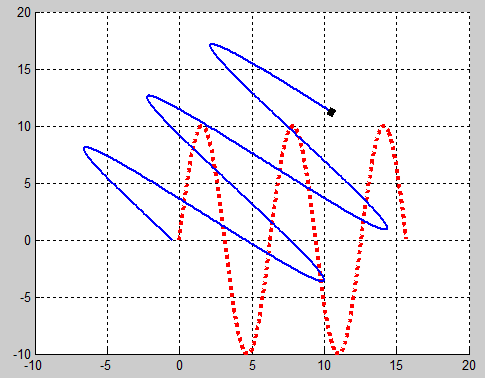
\includegraphics[width=0.5\textwidth]{OpenZero}
\end{figure}

\begin{figure}[h!]
  \caption{Close Loop with Zero Error, without Noise}
  \centering
    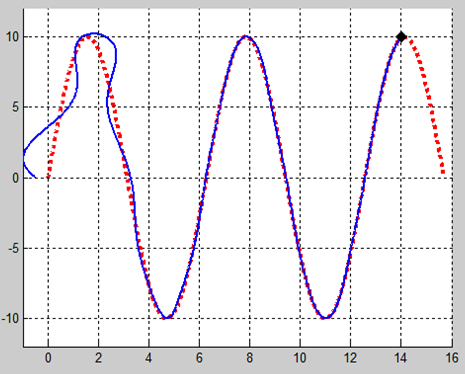
\includegraphics[width=0.5\textwidth]{CloseZero}
\end{figure}

\begin{figure}[h!]
  \caption{Open Loop with Noise, without Zero Error}
  \centering
    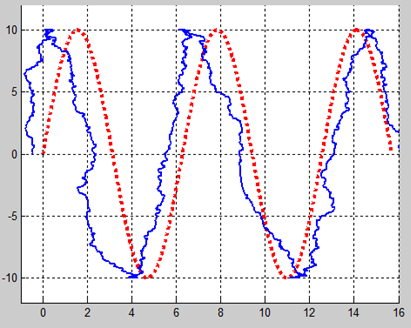
\includegraphics[width=0.5\textwidth]{OpenNoise}
\end{figure}

\begin{figure}[h!]
  \caption{Close Loop with Noise, without Zero Error}
  \centering
    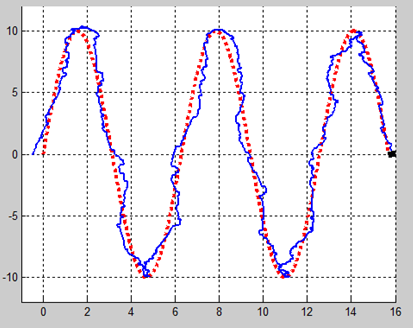
\includegraphics[width=0.5\textwidth]{CloseNoise}
\end{figure}

%%%%%%%%%%%%%%%%%%%%%%%%%%%%%%%%%%
\section{Conclusions \& Further Work}
Trajectory analysis of a differential robot was performed in this paper. The robot was provided with a reference trajectory to follow under noise free and noisy conditions
and the results were recorded. The robot kinematics were used and an error based state space was designed for the differential robot and a linear controller was designed to control the robot with
feedback. It was then provided with the same trajectories under noise and noise free conditions and results were recorded. From the simulation results it was concluded that
that robot swayed far away form the reference path under non ideal conditions but was able to track the path with satisfactory accuracy.It was further noted that if the open loop robot was not in the correct pose at the start the it drifted very far away from the given trajectory. However, in the closed loop case,
the robot drifted off but came back close to the reference path minimizing the error between the reference and actual path.Further future work can be carried on this to
control the differential robot with a  non linear controller. 

\bibliography{mybib}{}
\bibliographystyle{IEEEtran}

% that's all folks
\end{document}
